\section{Design Model}


%%%%%%%%%%%%%%%%%%%%%%%%%%%%%%%%%%%%%%%
\subsection{Components and Overall Structure}
Structural design model.
see \ref{fig:designmodel1}. Application is in Java. Knowledge mostly in Jess and
for a part in Java (see section on inferences). Java application starts jess
engine with working memory.

In the working memory are the domain rules, facts
that represent inferential knowledge of car, and the domain parts, knowledge
about the current status of parts of the car. Domain rules are not modified over
a run of the program, domain parts are modified.

Information from the app goes to jess by asserting
support facts, these are then interpeted as modifications of domain parts.
Inferences made by Jess go to the app by queries made by the app.

The Jess parts is divided in a engine and a domain part. The domain rules and
domain parts are implementations of templates supplied by the engine. The
engines inferences makes forward and backward reasonings from these rules and
parts. The domain rules and parts can be substituted by rules and parts from a
different domain while keeping the engine. The rules might be understandable by an
expert or user, our car repair hobbyist does. The complexity of the inferences
made by the engine are not visible in the domain part.

\begin{figure}[htbp]
    \centering
    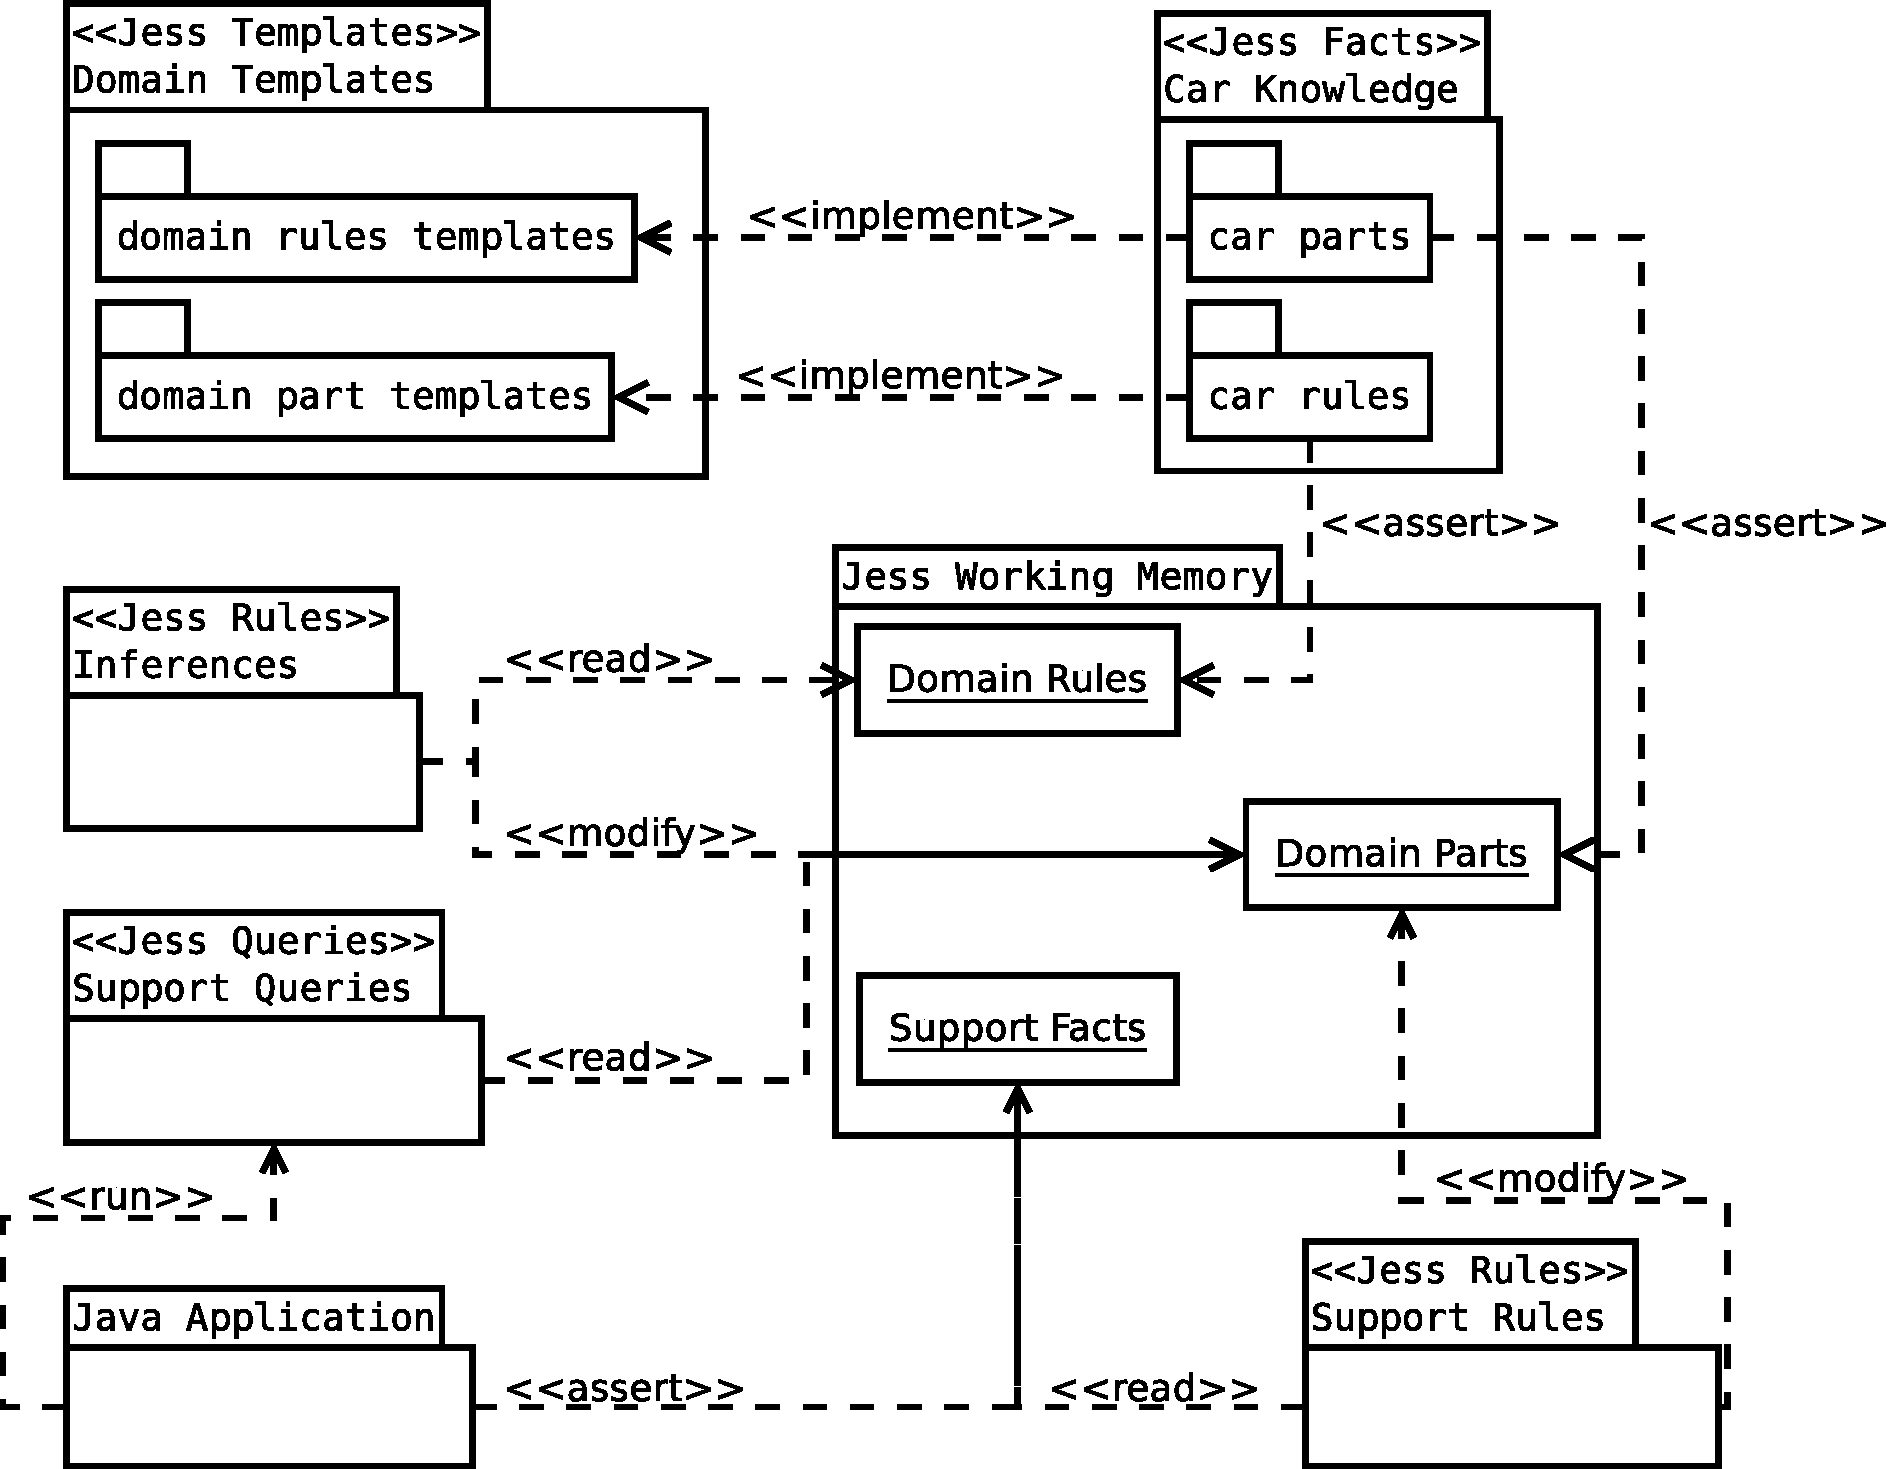
\includegraphics[width=1.00\textwidth]{designmodel-packages.pdf}
    \caption{The designmodel of our system}
    \label{fig:designmodel1}
\end{figure}

%%%%%%%%%%%%%%%%%%%%%%%%%%%%%%%%%%%%%%%
\subsection{Components and Overall Structure}

%%%%%%%%%%%%%%%%%%%%%%%%%%%%%%%%%%%%%%%
% Knowledge Management and Modelling Final
% Tycho Bismeijer
% Joost Huizinga
% 10 feb 2011

\documentclass[a4paper,10pt]{article}

\usepackage{array}
\usepackage{lmodern}
\usepackage{graphicx}

\graphicspath{{../diagrams/}{}}

% Voor de CommonKADS worksheets
\def\pbs#1{\let\temp=\\#1\let\\=\temp}
\def\colleft{\pbs\raggedright\hspace{0pt}}

\title{The Car Repair Assistant}
\author{
Joost Huizinga (1557017)\\
Tycho Bismeier (1615440)}
\date{\today}

\begin{document}

\section{Design}
\subsection{Inferences}
\subsubsection{Knowledge base}
Most inferences use the causal-model knowledge base. This knowledge base is mainly implemented in the file \textbf{car-rules.jess}. In this file there is a list of facts. Every facts implements a rule from the causal-model knowledge base. There are four types of facts: causes-to-wire, causes-from-wire, causes-from-2wires and causes-feature. These types correspond to the rule type found in the causal model knowledge base with the exception of causes-from-2wires which is a special case of the causes-from-wire rule type. Below is an example of a causes-to-wire fact.

\begin{verbatim}
(causes-to-wire
   (faulty-comp-type battery)
   (faulty-comp-state empty)
   (wire-state no-power)
)
\end{verbatim}

This fact should be interpreted as the rule: if a component is a battery and this battery is empty then any wire connected to it will have no power. For actual reasoning these facts are used by jess rules defined in other files. This approach was chosen because it grants flexibility. For example, the addition of one rule will enable all forward reasoning for causes-to-wire. The addition one additional rule will then enable all backward reasoning for causes-to-wire. If we implemented these rules directly as jess rules then we had to create two rules for every fact in this file.


\subsubsection{Cover}
The cover step has been divided into two parts. The first part creates a list of single component hypothesis, which we will call \emph{basic hypothesis}. The second part expands some of these basic hypothesis into multi component hypothesis, which we will call \emph{composed hypothesis}.

The first part is implemented in jess, in the file \textbf{cover-rules.jess}, and uses the causal-model knowledge base. The reasoning process will start at a complaint and it will then reason backwards through the components listing all possible causes for the complaint. One of the rules used in this process is shown below.

\begin{verbatim}
(defrule causes-feature-cover
"If a faulty state of a component causes an observed complaint, 
that component might be in that state"
   (observable
      {observed == TRUE}
      {complaint == TRUE}
      (id ?oid)
   )
   (causes-feature
      {observable == ?oid}
      (component ?cid)
      (component-state ?cstate)
   )
   ?c <- (component
      {id == ?cid}
      (possible-states $?ps&~:(member$ ?cstate ?ps))
      (impossible-states $?ips&~:(member$ ?cstate ?ips))
   )
   =>
   (modify ?c
      (possible-states (create$ ?ps ?cstate))
   )
)
\end{verbatim}

The rule above has four parts. The first part triggers when there is an observable that was marked as a complaint. The second part triggers when there exists a `rule' (remember that these rules are implemented as jess facts) that links this observable with a component and a state. The third part checks whether this component already has this state as a possible or impossible state. The fourth part is the consequent and adds the state to the possible-states of the component.

The other rules will propagate possible states in a similar manner such that, at the end of the reasoning process, every component that could potentially be the cause of the complaint has a possible state that would cause this component to malfunction. Then a query will collect all component-state combinations and each of these combinations becomes a hypothesis.

While this seems to be a perfectly reasonable way to find hypothesis there is one problem: there might be a merge in the reasoning trace. A merge is a component that has two inputs and that gives power when one of its inputs provides power, functioning as a logical OR. If such a component has no power then this is because there are two components that do not provide power two the merge. As such, the hypothesis now involves two components. Because of implementation problems this issue has not been addressed in jess. Instead it has been solved in the java code and it comprises the second part of cover.



The second part of cover expands the basic hypothesis when the hypothesis alone is not enough to explain the complaint. This part has been coded in java and is shown below.

\begin{verbatim}
private List<Hypothesis> expandHypothesis(List<Hypothesis> allHypothesis) {
    ...

    for(int i=0; i<allHypothesis.size(); i++){
        currentHypothesis = allHypothesis.get(i);

        if(currentHypothesis.directCause()){
            result.add(allHypothesis.get(i));
        } else {
            currentHypothesis.maxIndex = basicHypothesis.size();
            basicHypothesis.add(currentHypothesis);
            candidateHypothesis.add(currentHypothesis); 
        }
    }
\end{verbatim}

The first part creates a list of which hypothesis should be expanded, namely those that would not by themselves cause the complaint. Those that do cause the complaint by themselves are fine hypothesis and are immediatly added to the result. Note that, in order to find out if an hypothesis would cause the complaint, the causal model is used again, only 

The hypothesis that are selected for expansion are added to two different lists: the basic hypothesis list and the candidate hypothesis list. The basic hypothesis list will be used to expand other hypothesis. The candidate hypothesis list is the list of hypothesis to be expanded and it will grow when  hypothesis need to be expanded more then once.

\begin{verbatim}
        //Expand the candidate hypothesis
        while(candidateHypothesis.peek() != null){
            //Get the first hypothesis
            currentHypothesis = candidateHypothesis.pop();
            for(int j=currentHypothesis.maxIndex; j<basicHypothesis.size(); j++){
                //For each basic hypothesis that we have not tried with this combination
                //Create a new composed hypothesis by expanding the candidate with the basic hypothesis
                newHypothesis = currentHypothesis.clone();
                newHypothesis.add(basicHypothesis.get(j));

                if(newHypothesis.directCause()){
                    //If the new hypothesis is a direct cause then a new composed hypothesis has been found
                    //Add it to the result
                    result.add(newHypothesis);
                } else {
                    //If the new hypothesis is not a direct cause then it might need further expanding.
                    //Check whether new information was gained with the composed hypothesis by
                    //checking whether the new hypothesis causes more state changes then
                    //the two previous hypothesis combined
                    if((currentHypothesis.nrStateChanges() + basicHypothesis.get(j).nrStateChanges() < newHypothesis.nrStateChanges())){
                        //If new information was gained then the new hypothesis
                        //should get further expanded
                        candidateHypothesis.add(newHypothesis);
                    }
                }
            }
        }

        return result;
    }

\end{verbatim}

\end{document}



